%%%%%%%%%%%%%%%%%%%%%%%%%%%%%%%%%%%%%%%%%%%%%%%%%%%%%%%%%%%%%%%%%%%%%%%%%%%%%%%%%%%
%%                 PŘÍLOHA - TESTOVÁNÍ                                           %%
%%%%%%%%%%%%%%%%%%%%%%%%%%%%%%%%%%%%%%%%%%%%%%%%%%%%%%%%%%%%%%%%%%%%%%%%%%%%%%%%%%%
\chapter[Porovnání rychlosti algoritmů]{Porovnání rychlosti algoritmů po~použití prostorových indexů}
\label{priloha-testovani}

Porovnání bylo provedeno měřením času výpočtu pro daný algoritmus
pro~různá vstupní data a~dvě různě zvolené toleranční vzdálenosti.
Pro každou konfiguraci (algoritmus, vstupní data, toleranční vzdálenost)
byl měřen čas výpočtu celkem desetkrát bez použití a~desetkrát s~použitím
prostorových indexů. Cílem bylo určení změny rychlosti algoritmů zavedením
prostorových indexů. Testování bylo provedeno na~přenosném počítači 
s~parametry uvedenými v~tabulce \ref{tab:parametry}. 

\vspace{10pt}
\begin{table}[H]
 \centering
  \caption{Parametry počítače využitého pro testování}
\begin{tabular}{|l|l|}
\hline
 typ počítače & \textit{HP ProBook 6450b} \\
\hline
 paměť & \textit{4 GiB} \\
\hline
 procesor &\textit{Intel® Core™ i5 CPU M 450 @ 2.40GHz $\times$ 4 }\\
\hline
 operační systém &\textit{Ubuntu 12.04 LTS, 64 bit}\\
\hline
\end{tabular}
  \label{tab:parametry}
\end{table}

\vspace{10pt}
V~následujících tabulkách jsou uvedeny časy zpracování pro danou upravovanou
a~referenční vrstvu (tabulka \ref{tab:vstup}) a~zvolenou toleranční vzdálenost. 
Časy jsou uváděny v~sekundách. 
% První číslo uvádí čas zpracování bez prostorových indexů, druhé při jejich použití

\vspace{10pt}
\begin{table}[H]
 \centering
  \caption{Vstupní vrstvy}
\begin{tabular}{|l|l|l|}
\hline
 typ dat & referenční vrstva & upravovaná vrstva \\
\hline
\hline
 polygony & vyber\_obce & vyber\_CR \\
 linie & zel1 & zel2 \\
 \hline
\end{tabular}
  \label{tab:vstup}
\end{table}


% \begin{table}
% \centering
%   \begin{tabular}{|c|cc|cc|cc|cc|}
% \hline
% data & \multicolumn{4}{c|}{polygony} & \multicolumn{4}{c|}{linie} \\
% \hline
% tol. vzdálenost &  \multicolumn{2}{c|}{100 m} & \multicolumn{2}{c|}{10 000 m} & \multicolumn{2}{c|}{100 m} & \multicolumn{2}{c|}{10 000 m} \\
% \hline
% \hline
% 1	&	19,89	&	0,78	&	23,52	&	0,69	&	4,41	&	0,45	&	5,16	&	0,47	\\
% 2	&	19,83	&	0,75	&	23,00	&	0,72	&	4,41	&	0,51	&	4,44	&	0,49	\\
% 3	&	21,98	&	0,69	&	23,63	&	0,76	&	4,43	&	0,48	&	4,66	&	0,50	\\
% 4	&	22,09	&	0,72	&	21,40	&	0,71	&	4,89	&	0,50	&	5,18	&	0,45	\\
% 5	&	21,99	&	0,77	&	21,50	&	0,78	&	4,90	&	0,48	&	5,20	&	0,48	\\
% 6	&	19,89	&	0,82	&	22,59	&	0,76	&	4,89	&	0,49	&	4,67	&	0,49	\\
% 7	&	19,76	&	0,90	&	22,59	&	0,70	&	4,91	&	0,43	&	5,17	&	0,50	\\
% 8	&	19,77	&	0,69	&	22,21	&	0,78	&	4,89	&	0,47	&	5,15	&	0,44	\\
% 9	&	21,95	&	0,68	&	23,61	&	0,69	&	4,45	&	0,43	&	4,92	&	0,51	\\
% 10	&	22,00	&	0,76	&	21,97	&	0,84	&	4,48	&	0,44	&	4,68	&	0,49	\\
% \hline																	
% \hline																	
% průměr	&	20,92	&	0,76	&	22,60	&	0,74	&	4,67	&	0,47	&	4,92	&	0,48	\\
% \hline
% \end{tabular}
%   \caption{Čas zpracování s~a~bez prostorových indexů pro \texttt{Vertex\-Snapper}}
%   \label{tab:vs-rychlost}
% \end{table}

\begin{table}
 \centering
  \small
   \caption{\texttt{Vertex\-Snapper} -
	    čas zpracování bez prostorových indexů}
  \begin{tabular}{|c|c|c|c|c|}
   \hline
      & \multicolumn{2}{c|}{polygony} & 
 	\multicolumn{2}{c|}{linie} \\
   \hline
    id  &  ~~100 m~ & 10 000 m & ~~~100 m & 10 000 m\\
   \hline
   \hline
 1  & 19.89 & 23.52 & 4.41 & 5.16 \\ 
 2  & 19.83 & 23.00 & 4.41 & 4.44 \\
 3  & 21.98 & 23.63 & 4.43 & 4.66 \\
 4  & 22.09 & 21.40 & 4.89 & 5.18 \\
 5  & 21.99 & 21.50 & 4.90 & 5.20 \\
 6  & 19.89 & 22.59 & 4.89 & 4.67 \\
 7  & 19.76 & 22.59 & 4.91 & 5.17 \\
 8  & 19.77 & 22.21 & 4.89 & 5.15 \\
 9  & 21.95 & 23.61 & 4.45 & 4.92 \\
 10 & 22.00 & 21.97 & 4.48 & 4.68 \\
   \hline
   \hline
   průměr & 20.92 & 22.60 & 4.67 & 4.92 \\
   \hline
  \end{tabular}
   \label{tab:vs-bez}
\end{table}
 
\begin{table}
 \centering
  \small
   \caption{\texttt{Vertex\-Snapper} -
	    čas zpracování s prostorovými indexy}
  \begin{tabular}{|c|c|c|c|c|}
   \hline
      & \multicolumn{2}{c|}{polygony} & 
 	\multicolumn{2}{c|}{linie} \\
   \hline
    id  &  ~~100 m~ & 10 000 m & ~~~100 m & 10 000 m\\
   \hline
   \hline
   1  & 0.78 & 0.69 &  0.45 & 0.47 \\
   2  & 0.75 & 0.72 &  0.51 & 0.49 \\
   3  & 0.69 & 0.76 &  0.48 & 0.50 \\
   4  & 0.72 & 0.71 &  0.50 & 0.45 \\
   5  & 0.77 & 0.78 &  0.48 & 0.48 \\
   6  & 0.82 & 0.76 &  0.49 & 0.49 \\
   7  & 0.90 & 0.70 &  0.43 & 0.50 \\
   8  & 0.69 & 0.78 &  0.47 & 0.44 \\
   9  & 0.68 & 0.69 &  0.43 & 0.51 \\
   10 & 0.76 & 0.84 &  0.44 & 0.49 \\
   \hline
   \hline
   průměr & 0.76 & 0.74 & 0.47 & 0.48 \\
   \hline
  \end{tabular}
   \label{tab:vs-s}
\end{table}
 
\begin{table}
 \centering
  \small
   \caption{\texttt{Coverage\-Alignment} - 
	    čas zpracování bez prostorovýczh indexů}
  \begin{tabular}{|c|c|c|c|c|}
   \hline
      & \multicolumn{2}{c|}{polygony} & 
 	\multicolumn{2}{c|}{linie} \\
   \hline
    id  &  ~~100 m~ & ~1 000 m & ~1 000 m & 10 000 m\\
   \hline
   \hline
 1  & 38.75 & 37.68 & 10.02 & 11.45 \\ 
 2  & 38.55 & 37.93 & 10.36 & 8.99  \\
 3  & 38.51 & 37.44 & 10.24 & 10.06 \\
 4  & 41.60 & 36.95 & 11.22 & 10.41 \\
 5  & 34.02 & 41.81 & 10.04 & 11.22 \\
 6  & 40.31 & 38.55 & 10.44 & 10.02 \\
 7  & 38.77 & 41.39 & 11.21 & 9.88 \\
 8  & 38.54 & 36.79 & 10.09 & 11.30 \\
 9  & 37.69 & 39.69 & 9.67  & 11.32 \\
 10 & 36.72 & 41.60 & 11.67 & 10.29 \\
   \hline
   \hline
   průměr & 38.35 & 38.98 & 10.51 & 10.49 \\
   \hline
  \end{tabular}
   \label{tab:ca-bez}
\end{table}
 
\begin{table}
 \centering
  \small
   \caption{\texttt{Coverage\-Alignment} - 
	    čas zpracování s~prostorovými indexy}
  \begin{tabular}{|c|c|c|c|c|}
   \hline
      & \multicolumn{2}{c|}{polygony} & 
 	\multicolumn{2}{c|}{linie} \\
   \hline
    id  &  ~~100 m~ & ~1 000 m & ~1 000 m & 10 000 m\\
   \hline
   \hline
 1  & 1.05 & 1.82 &  0.73 & 3.99 \\
 2  & 1.13 & 1.78 &  0.69 & 3.98 \\
 3  & 1.14 & 1.66 &  0.68 & 4.01 \\
 4  & 1.04 & 1.65 &  0.77 & 4.37 \\
 5  & 1.04 & 1.79 &  0.78 & 4.39 \\
 6  & 1.03 & 1.79 &  0.70 & 3.96 \\
 7  & 1.06 & 1.87 &  0.69 & 3.99 \\
 8  & 1.12 & 1.84 &  0.77 & 3.99 \\
 9  & 1.02 & 1.80 &  0.68 & 4.39 \\
 10 & 1.14 & 1.76 &  0.70 & 4.38 \\
   \hline
   \hline
   průměr & 1.08 & 1.78 & 0.72 & 4.15 \\
   \hline
  \end{tabular}
   \label{tab:ca-s}
\end{table}
 
\normalsize

%%%%%%%%%%%%%%%%%%%%%%%%%%%%%%%%%%%%%%%%%%%%%%%%%%%%%%%%%%%%%%%%%%%%%%%%%%%%%%%%%%%
%%                 PŘÍLOHA - UML DIAGRAMY TŘÍD                                   %%
%%%%%%%%%%%%%%%%%%%%%%%%%%%%%%%%%%%%%%%%%%%%%%%%%%%%%%%%%%%%%%%%%%%%%%%%%%%%%%%%%%%
\chapter{UML diagramy tříd}
\label{priloha-diagramy}

Následující UML diagramy zobrazují třídy spojené s~jednotlivými 
algoritmy a~jejich nejdůležitější atributy a~metody.

  \begin{figure}[hbt]
    \centering
      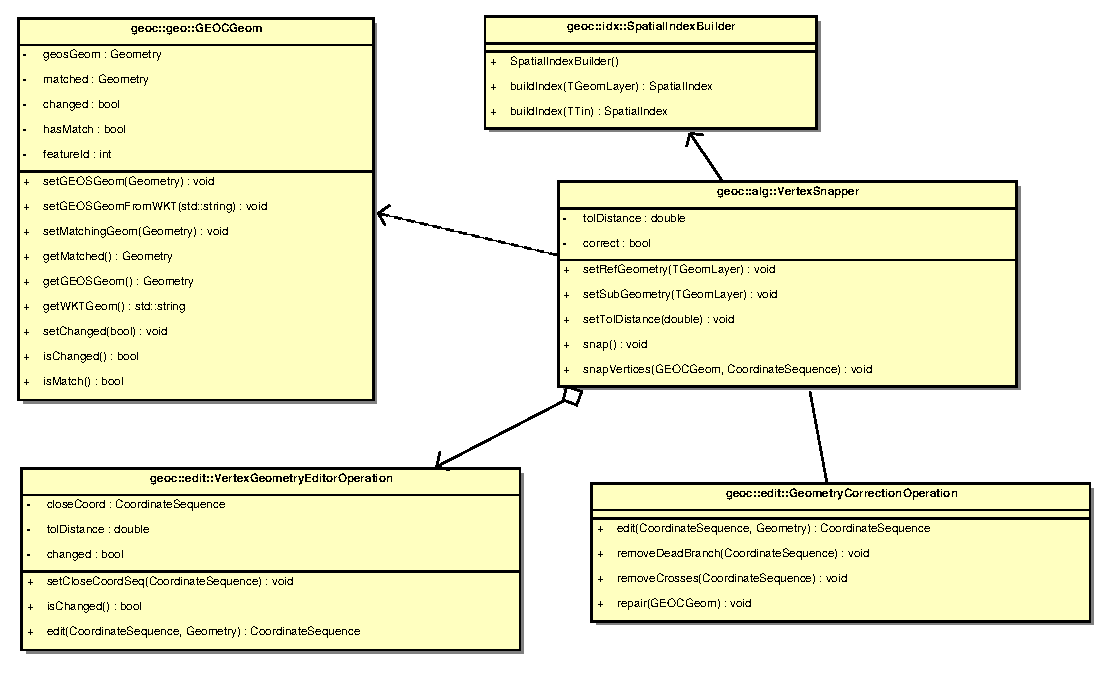
\includegraphics[width=420pt]{./pictures/uml-vs.pdf}
      \caption{UML diagram tříd pro VertexSnapper}
      \label{fig:uml-vs}
  \end{figure}

  \begin{figure}[hbt]
    \centering
      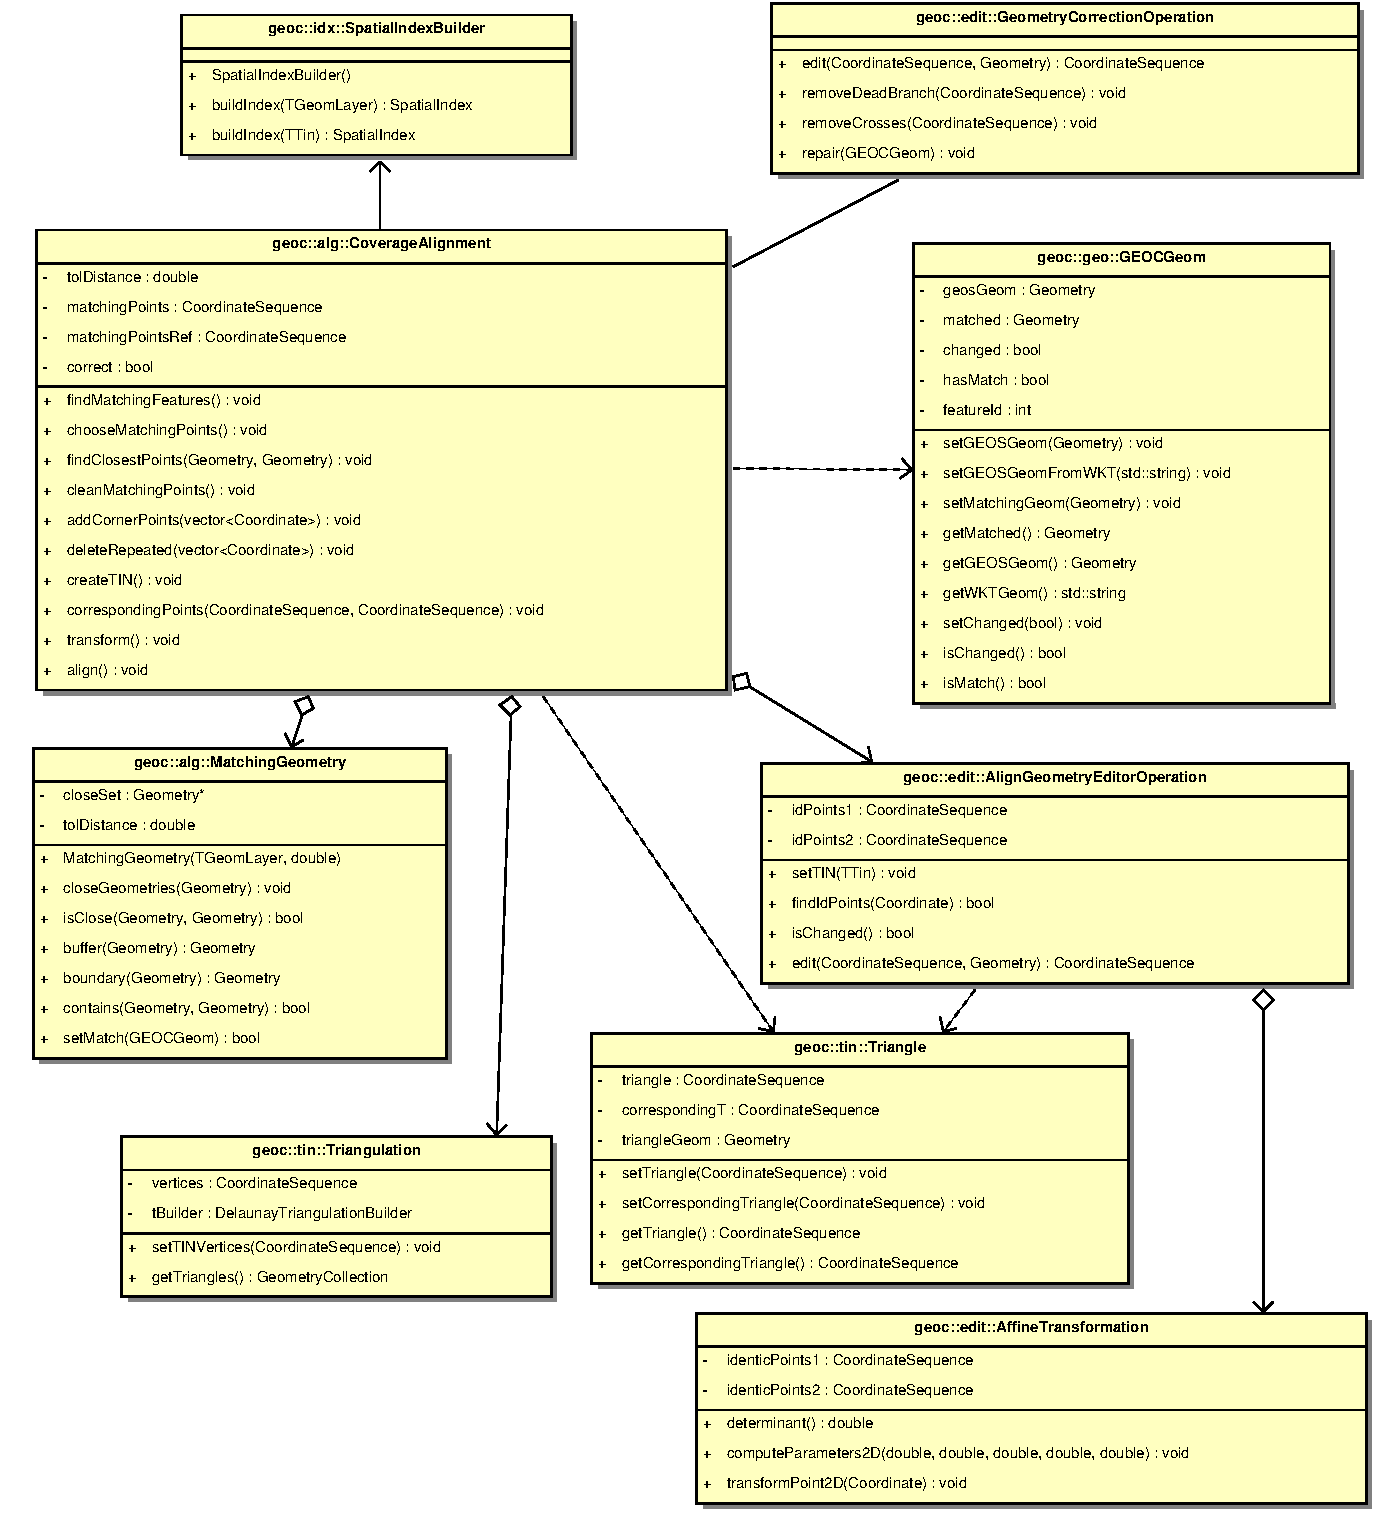
\includegraphics[width=420pt]{./pictures/uml-ca.pdf}
      \caption{UML diagram tříd pro CoverageAlignment}
      \label{fig:uml-ca}
  \end{figure}

  \begin{figure}[hbt]
    \centering
      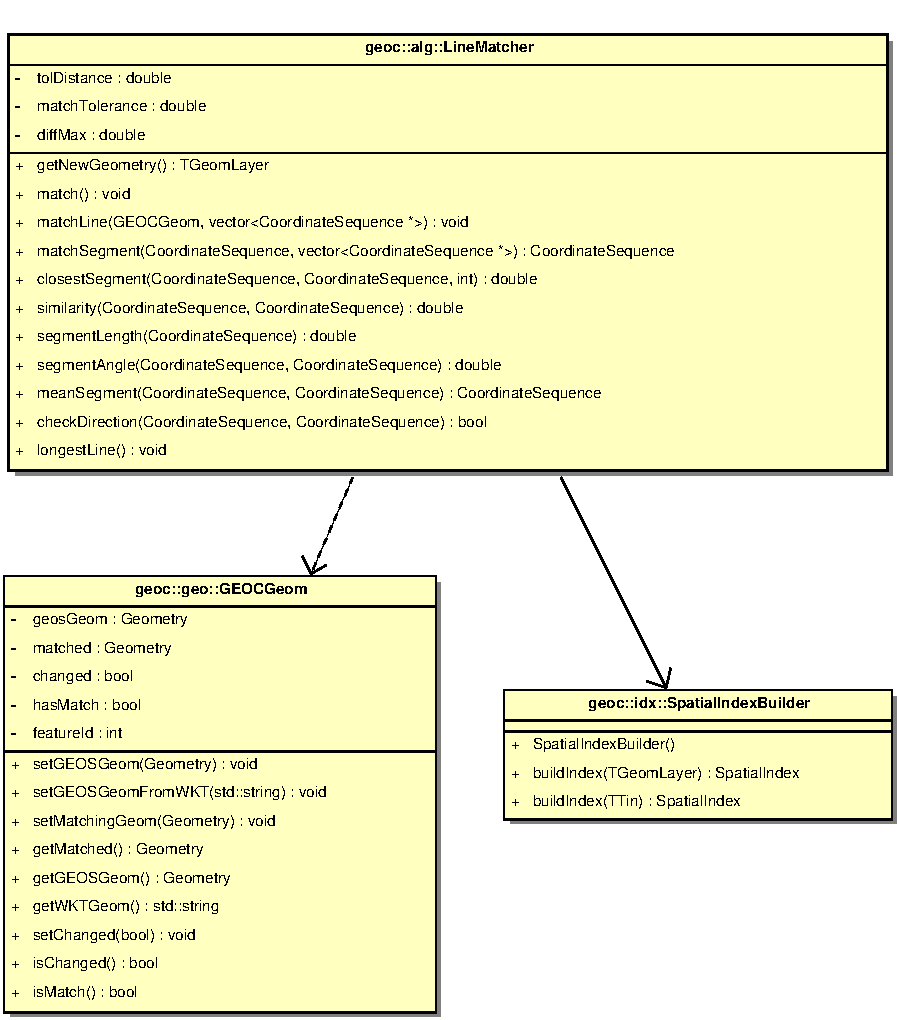
\includegraphics[width=420pt]{./pictures/uml-lm.pdf}
      \caption{UML diagram tříd pro LineMatcher}
      \label{fig:uml-lm}
  \end{figure}

%%%%%%%%%%%%%%%%%%%%%%%%%%%%%%%%%%%%%%%%%%%%%%%%%%%%%%%%%%%%%%%%%%%%%%%%%%%%%%%%%%%
%%                 PŘÍLOHA - UŽIVATELSKÁ PŘÍRUČKA                                %%
%%%%%%%%%%%%%%%%%%%%%%%%%%%%%%%%%%%%%%%%%%%%%%%%%%%%%%%%%%%%%%%%%%%%%%%%%%%%%%%%%%%
\chapter{Uživatelská příručka}
\label{priloha-prirucka}

Tato příručka je psána pro použití modulu \textit{Conflate} s~Quantum GIS 1.9.0 , 
v~jiných verzích se může způsob načtení modulu, popř. i~jiné činnosti mírně lišit.

\section{Instalace}
\label{prirucka-instalace}
Instalace ... %Je potřeba knihovna \textit{GEOC} ..

\section{Načtení zásuvného modulu}
\label{prirucka-nacteni}

Načtení zásuvného modulu lze provést ve~Správci zásuvných modulů.
\begin{center}
\textit{Zásuvné moduly~$\rightarrow$~Spravovat~zásuvné~moduly... 
(Plugins~$\rightarrow$~Plugin Manager...)}
\end{center}
Zde je třeba zaškrtnout \textit{Conflate Plugin}. Po~provedení tohoto kroku by se 
měla objevit ikonka modulu v~nástrojové liště a~také v~menu \textit{Zásuvné moduly}. 
Pokud se plugin nezobrazuje ve~Správci zásuvných modulů, je třeba nastavit cestu 
k~souboru~\textit{.so} v~\textit{Nastavení}.
\begin{center} 
\textit{Nastavení~$\rightarrow$~Volby~$\rightarrow$~Systém~$\rightarrow$~Cesty 
k~zásuvným modulům (Settings~$\rightarrow$~Options$\rightarrow$~System~$\rightarrow$
~Plugin paths)}
\end{center}


\section{Spuštění a nastavení dialogu}
\label{prirucka-spusteni}

\subsection{Výběr vstupních vrstev}
Před spuštěním dialogu \textit{Conflate} je třeba mít v~aktuálním projektu 
načteny vrstvy, které chceme zpracovávat. Pokud přidáme vrstvu až po~otevření
dialogu, lze ji načíst do~výběru vrstev tlačítkem \textit{Refresh}.
Po~otevření dialogu je třeba provést výběr \textbf{re\-ferenční vrstvy} 
(\textit{Reference Layer}) a~\textbf{upravované vrstvy} (\textit{Subject Layer}). 
Re\-ferenční vrstva je obvykla ta s~vyšší přesností, která se nebude měnit. 
Upravovanou vrstvu naopak chceme zarovnat k~vrstvě referenční. 
Obě vrstvy by měly být stejného geometrického typu (polygon~-~polygon, 
linie~-~linie, bod~-~bod).

\subsection{Metoda zpracování}
Dalším krokem je volba způsobu zpracování (\textit{Select the way of conflation}). 
Na~výběr jsou tyto metody, jejichž princip je naznačen na~obrázku \ref{fig:algorithms}.

\begin{itemize}
 \item \textbf{Přichycení vrcholů} (\textit{Snap Vertices}) - tato metoda vyhledá 
	blízké vrcholy z~obou datasetů a~změní polohu bodů upravované vrstvy tak, 
	aby odpovídala poloze blízkých bodů vrstvy referenční.
 \item \textbf{Zarovnání vrstev} (\textit{Coverage Alignment}) - princip této 
	metody je složitější. Na~rozdíl od~předchozí metody nepracuje s~jednotlivými
	body, ale s celými prvky. Upravuje i~některé prvky, k nimž neexistují 
	žádné odpovídající ve~vrstvě refe\-renční, a~to na~základě změny okolních 
	prvků. Je proto vhodnější zejména pro datasety, které mají rozdílný počet
	prvků. Obecně je možné s~touto metodou dosáhnout přesnějších a~často
	reálnějších výsledků, avšak na~úkor času zpraco\-vání.
 \item \textbf{Napasování linií} (\textit{Match lines} - tato metoda vyhledá
	odpovídající si úseky linií ze dvou různých vrstev. Takto nalezené
	páry zprůměruje a~vytvoří z~nich nové linie. Při volbě tohoto způsobu
	zpracování nezáleží na~tom, která vrstva je referenční a~která upravovaná.
	Napasování linií lze použít pouze na~dvojice liniových vrstev.
\end{itemize}

  \begin{figure}[H]
    \centering
      \def\svgwidth{400pt}
      \input{./pictures/algorithms.pdf_tex}
      \caption{Princip jednotlivých algoritmů}
      \label{fig:algorithms}
  \end{figure}

\subsection{Další nastavení}
Poté je třeba nastavit \textbf{toleranční vzdálenost} (\textit{Distance 
Tolerance}) v~jednotkách projektu. Tato vzdálenost udává, v~jaké maximální 
vzdálenosti mohou být odpovídající si prvky z~obou vrstev a~zároveň, jak 
moc se tedy může cílová vrstva měnit. V~ideálním případě by tato vzdálenost 
neměla přesahovat nejkratší segment geometrie všech prvků upravované vrstvy 
(tzn. nejkratší úsek linie, nejkratší stranu polygonu). Nevhodná volba této 
vzdálenosti může vést ke~vzniku nevalidních geometrií či nereálným výsledkům.

U~poslední metody (\textit{Match Lines}) se zviditelní ještě možnost nastavení
\textbf{kritéria podobnosti} \textit{Matching criterium}. Jedná se o~minimální 
podobnost dvou segmentů, která musí být dodržena pro jejich spárování. 
Tato hodnota se udává v~procentech. Při zadání $100 \%$ jsou výsledkem pouze 
naprosto totožné segmenty. Kritérium podobnosti se počítá na základě úhlu mezi 
segmenty, vzdálenosti jejich koncových bodů a~rozdílu jejich délek. 

Volba toleranční vzdálenosti a~metody zarovnání může výrazně ovlivnit rychlost 
zpracování, je proto doporučeno volit raději vždy menší vzdálenost a~jednodušší
metodu a~teprve po zobrazení výsledků případně parametry změnit.

Poslední nastavovanou možností je \textbf{automatická oprava geometrie}
 zaškrtnutím \textit{Try to repair invalid geometries}. Při této volbě se 
program pokusí opravit nově vzniklé nevalidní geometrie. Opravováno je pouze 
křížení úseků v~polygonu a~tzv. \uv{slepé větve}. Automatická oprava však 
může ovlivnit přesnost výsledku a~někdy i~vytvořit topologické chyby, proto 
je třeba ji používat opatrně. Při volbě \textit{Match Lines} není tato možnost
dostupná, jelikož uvedené situace nejsou u~liniových geometrií považovány
za~chybné.

Po~nastavení všech parametrů (včetně výstupní vrstvy - viz dále) se stisknutím 
tlačítka \textit{Process} spustí zpracování. 

\subsection{Výstupní vrstva}

Před spuštěním zpracování lze ještě nastavit název a~cestu, kam se má uložit
výsledný soubor. Upravená vrstva se vždy uloží jako nová vrstva ve~formátu 
\textit{shapefile}. Do~pole \textit{Output shapefile} lze zadat \textbf{cestu 
k~výstupnímu souboru}, popřípadě ji vybrat pomocí tlačítka \textit{Browse} 
(\textit{Procházet}) vpravo. 

Pokud zadáte pouze název výstupní vrstvy nebo toto pole necháte prázdné, 
uloží se nová vrstva do~aktuálního adresáře pod daným názvem nebo pod názvem
upravované vrstvy s~příslušným pořadovým číslem. 


\section{Výsledek}
\label{prirucka-vysledek}

Upravená vrstva se automaticky přidá do~otevřeného projektu v~QGISu.

V~dialogu zásuvného modulu se do~textového pole vlevo vypíše protokol o~zpracování.
Formát protokolu je popsán na~obrázku \ref{fig:protokol}.  

  \begin{figure}[H]
    \centering
      %\input{./pictures/protokol.pdf_tex}
      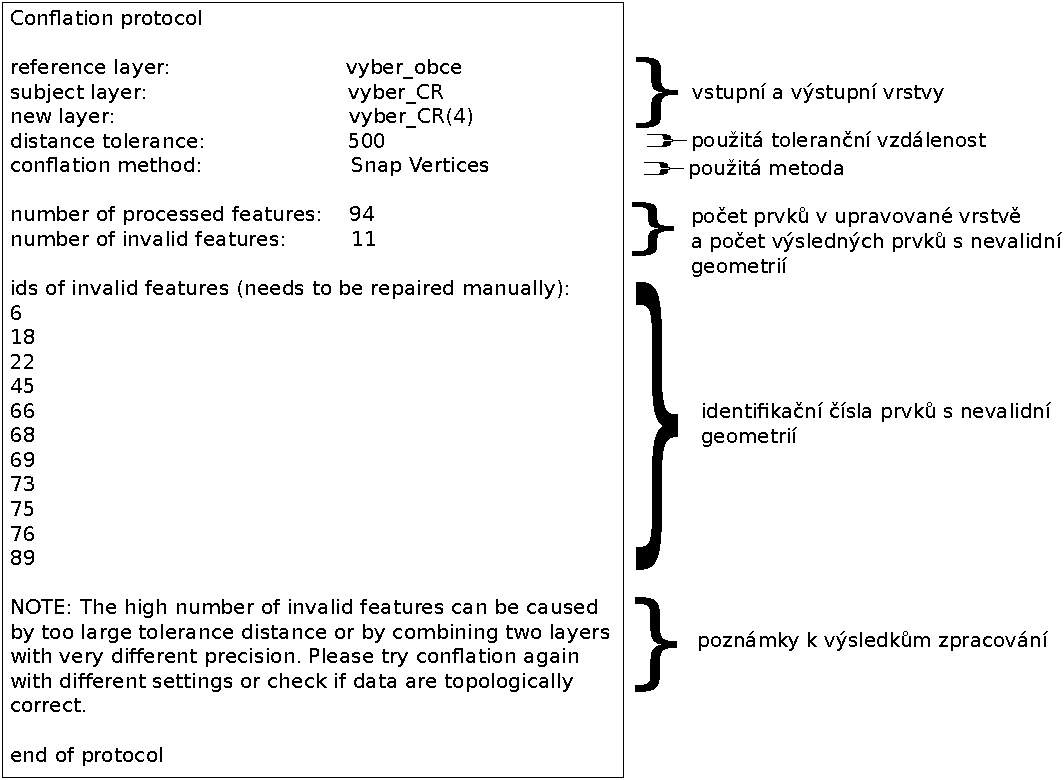
\includegraphics[width=420pt]{./pictures/protokol.pdf}
      \caption{Formát protokolu}
      \label{fig:protokol}
  \end{figure} 

Výsledkem zpracování mohou být i~nevalidní geometrie, jejichž identifikátory lze
nalézt v~protokolu. Proto jsou často nezbytné ještě závěrečné úpravy s~využitím
editačních nástrojů QGISu.


%%%%%%%%%%%%%%%%%%%%%%%%%%%%%%%%%%%%%%%%%%%%%%%%%%%%%%%%%%%%%%%%%%%%%%%%%%%%%%%%%%%
%%                 PŘÍLOHA - SCREENSHOTY                                         %%
%%%%%%%%%%%%%%%%%%%%%%%%%%%%%%%%%%%%%%%%%%%%%%%%%%%%%%%%%%%%%%%%%%%%%%%%%%%%%%%%%%%
\chapter{Screenshoty zásuvného modulu}
\label{priloha-screenshoty}

  \begin{figure}[H]
    \centering
      %\input{./pictures/protokol.pdf_tex}
      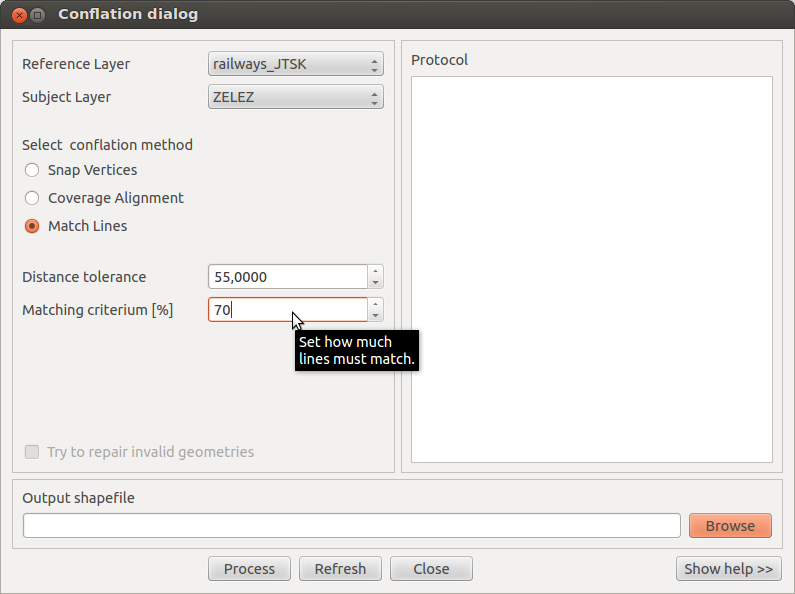
\includegraphics[width=360pt]{./pictures/dialog1.png}
      \caption{Dialog zásuvného modulu - nastavení}
      \label{fig:d1}
  \end{figure} 

  \begin{figure}[H]
    \centering
      %\input{./pictures/protokol.pdf_tex}
      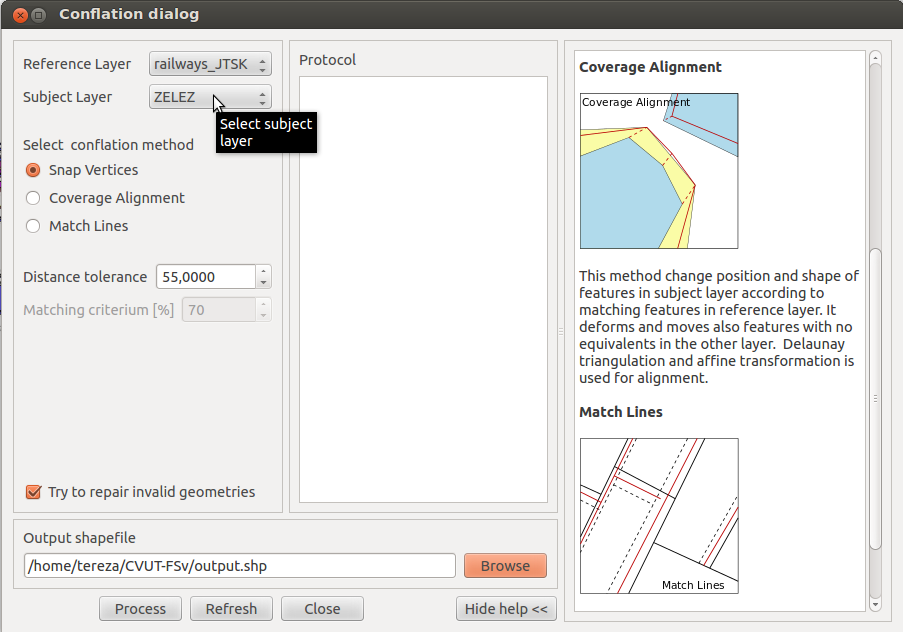
\includegraphics[width=360pt]{./pictures/dialog2.png}
      \caption{Dialog zásuvného modulu - nápověda}
      \label{fig:d2}
  \end{figure} 

  \begin{figure}[H]
    \centering
      %\input{./pictures/protokol.pdf_tex}
      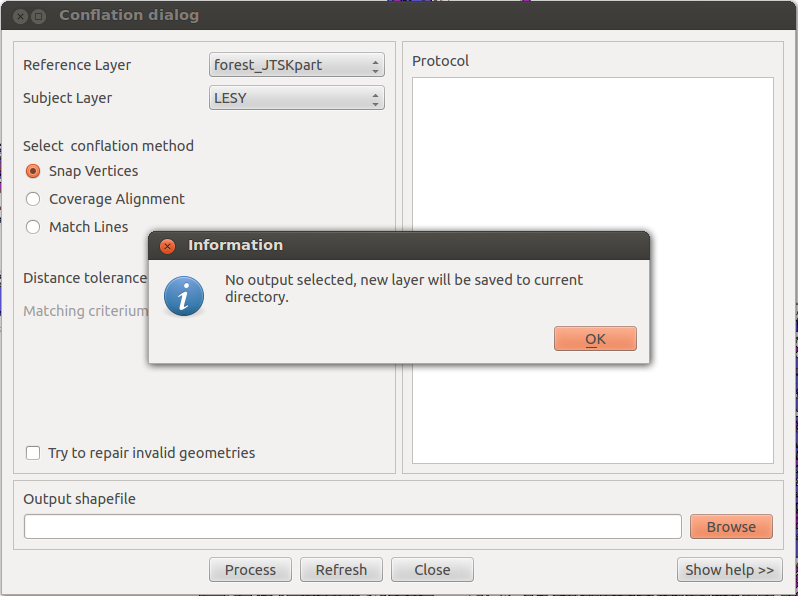
\includegraphics[width=360pt]{./pictures/dialog3.png}
      \caption{Dialog zásuvného modulu - upozornění}
      \label{fig:d3}
  \end{figure} 

  \begin{figure}[H]
    \centering
      %\input{./pictures/protokol.pdf_tex}
      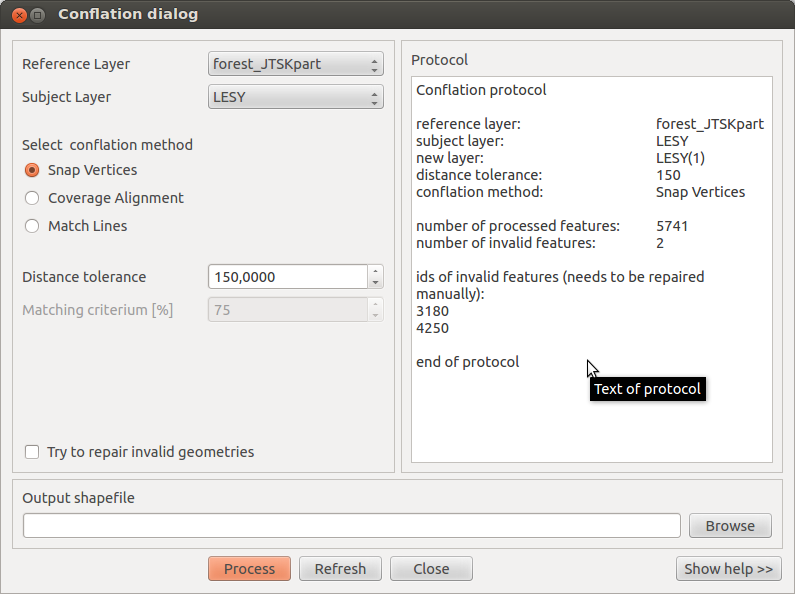
\includegraphics[width=360pt]{./pictures/dialog4.png}
      \caption{Dialog zásuvného modulu - protokol}
      \label{fig:d4}
  \end{figure} 

%%%%%%%%%%%%%%%%%%%%%%%%%%%%%%%%%%%%%%%%%%%%%%%%%%%%%%%%%%%%%%%%%%%%%%%%%%%%%%%%%%%
%%                 PŘÍLOHA - UKÁZKY                                              %%
%%%%%%%%%%%%%%%%%%%%%%%%%%%%%%%%%%%%%%%%%%%%%%%%%%%%%%%%%%%%%%%%%%%%%%%%%%%%%%%%%%%
\chapter{Ukázky zpracování dat}
\label{priloha-ukazky}

\section{VertexSnapper}
\label{ukazky-vs}

  \begin{figure}[H]
    \centering
      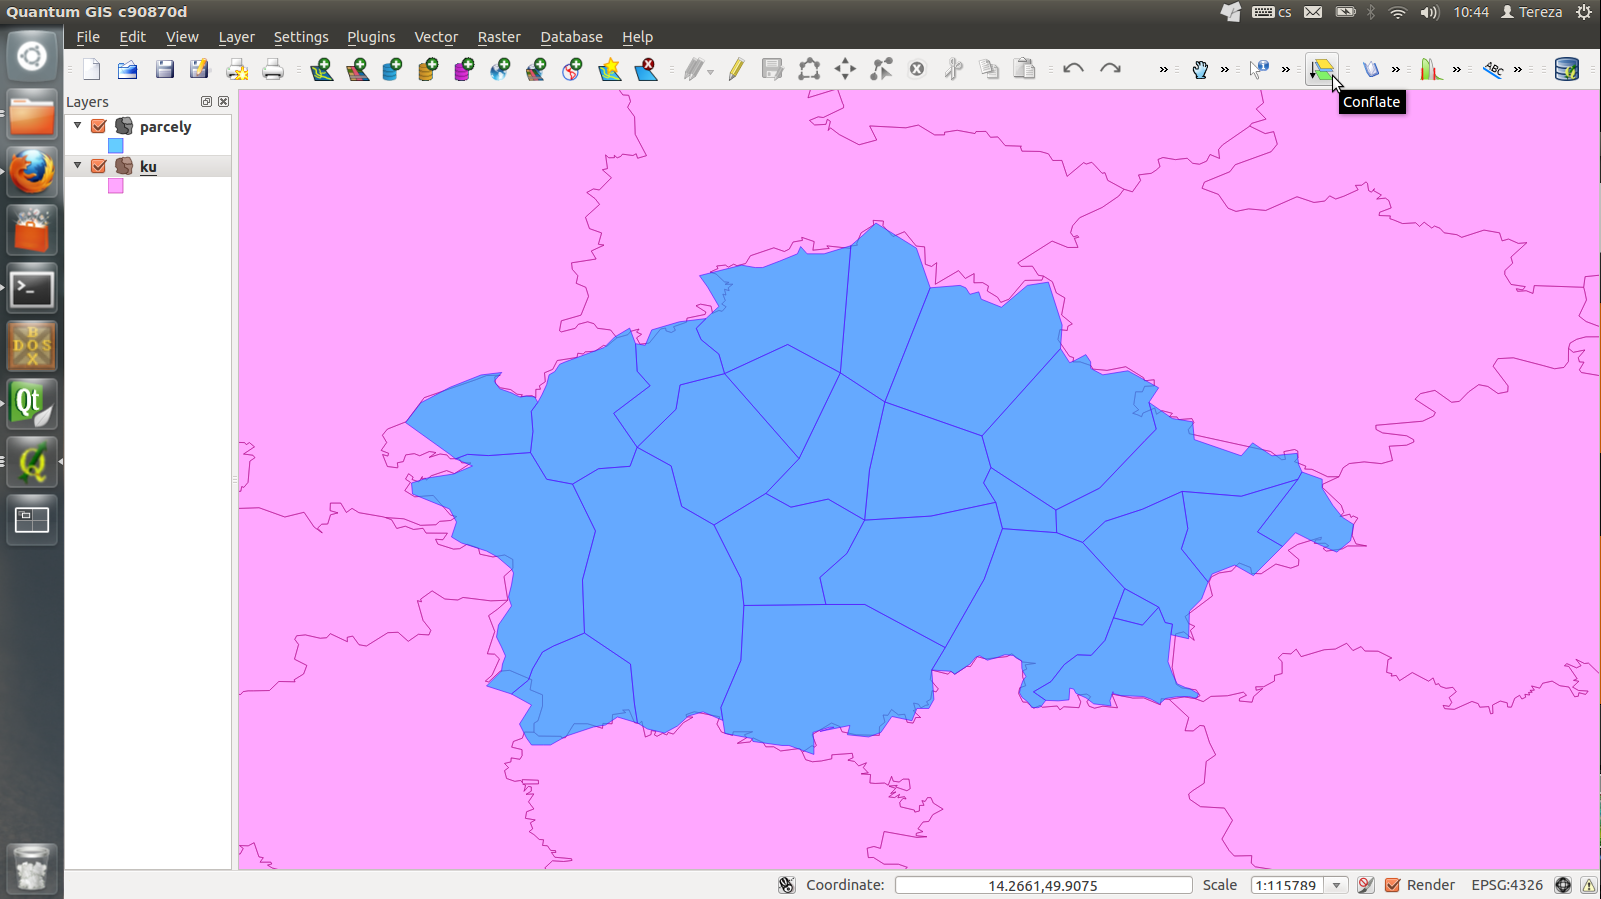
\includegraphics[width=400pt]{./pictures/test-vs1.png}
      \caption{VertexSnapper - vstupní data}
      \label{fig:vs1}
  \end{figure}

  \begin{figure}[H]
    \centering
      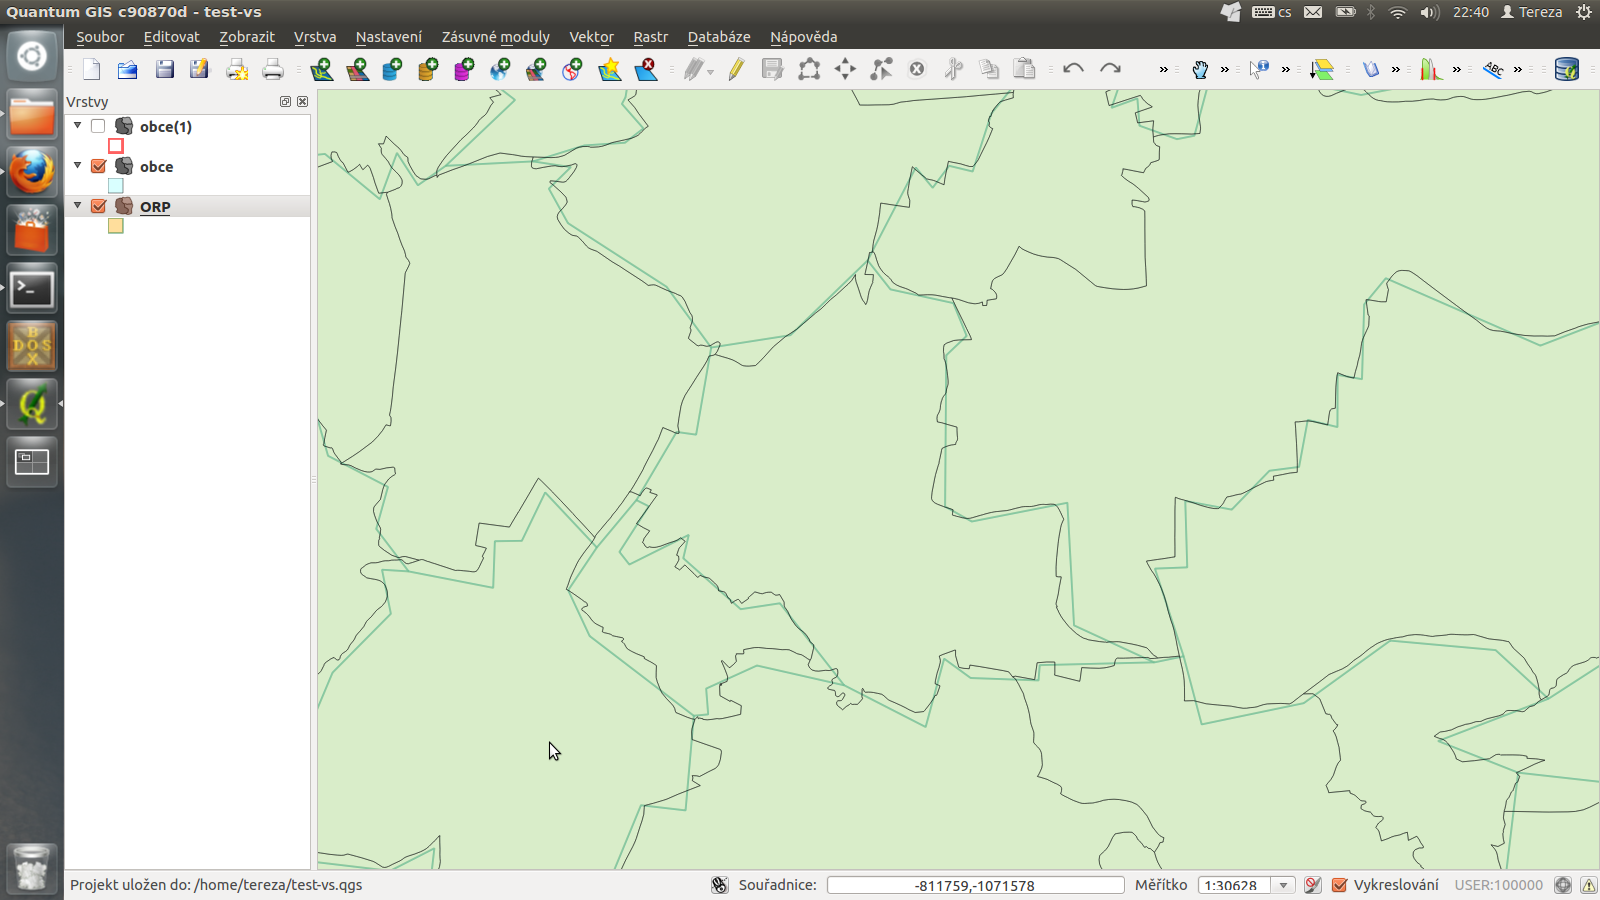
\includegraphics[width=400pt]{./pictures/test-vs2.png}
      \caption{VertexSnapper - před zpracováním}
      \label{fig:vs2}
  \end{figure}

  \begin{figure}[H]
    \centering
      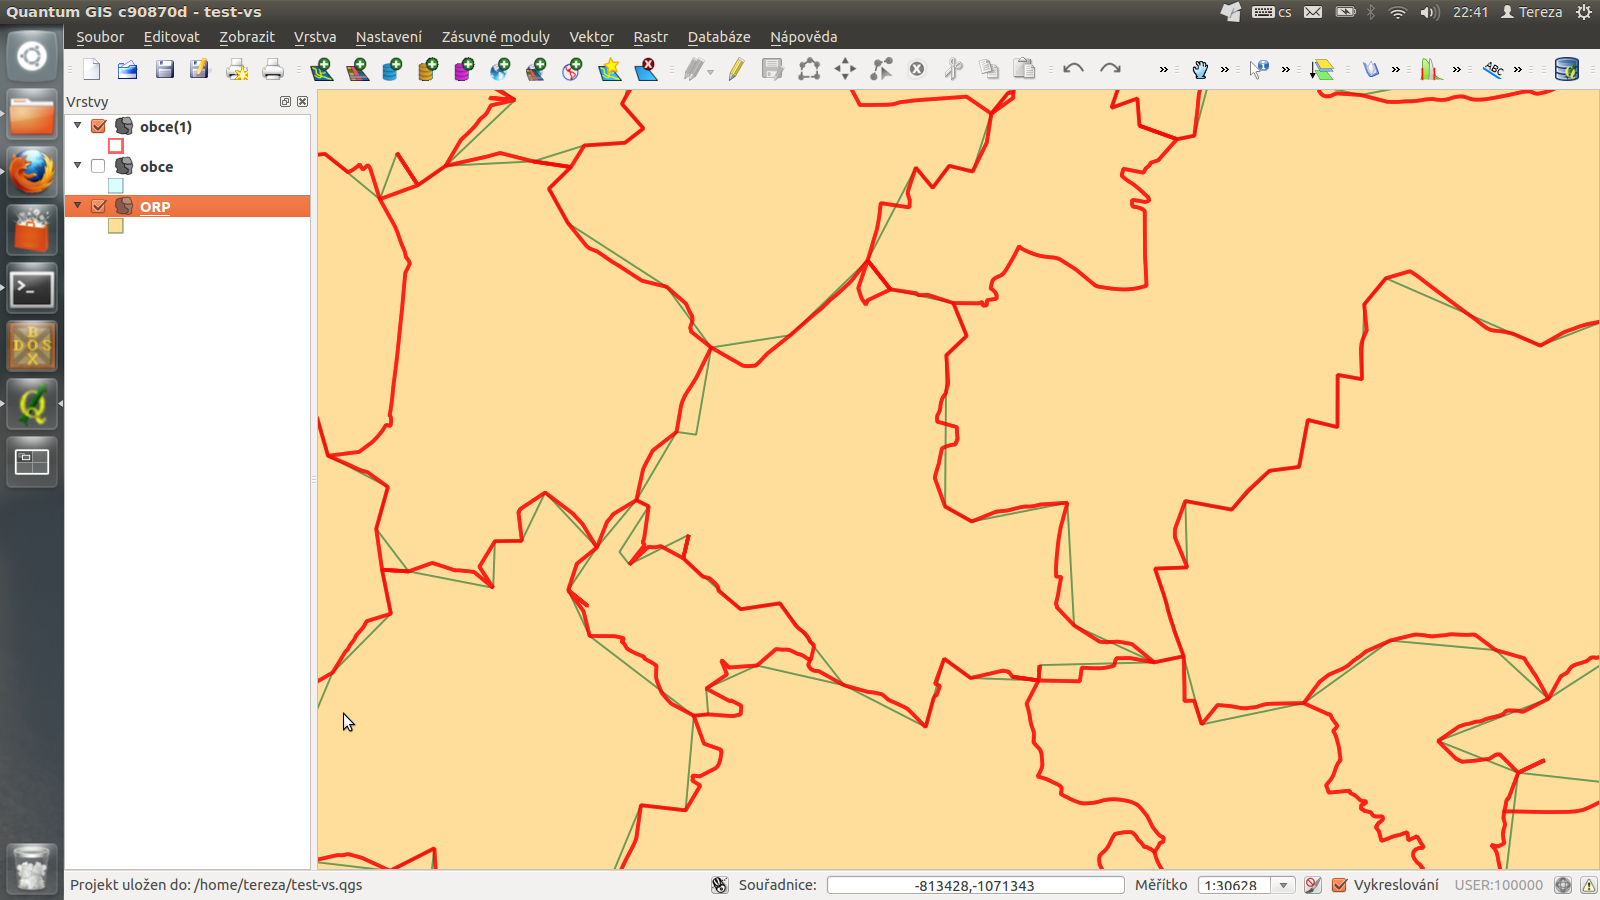
\includegraphics[width=400pt]{./pictures/test-vs3.png}
      \caption{VertexSnapper - po přichycení}
      \label{fig:vs3}
  \end{figure}


\section{CoverageAlignment}
\label{ukazky-ca}

  \begin{figure}[H]
    \centering
      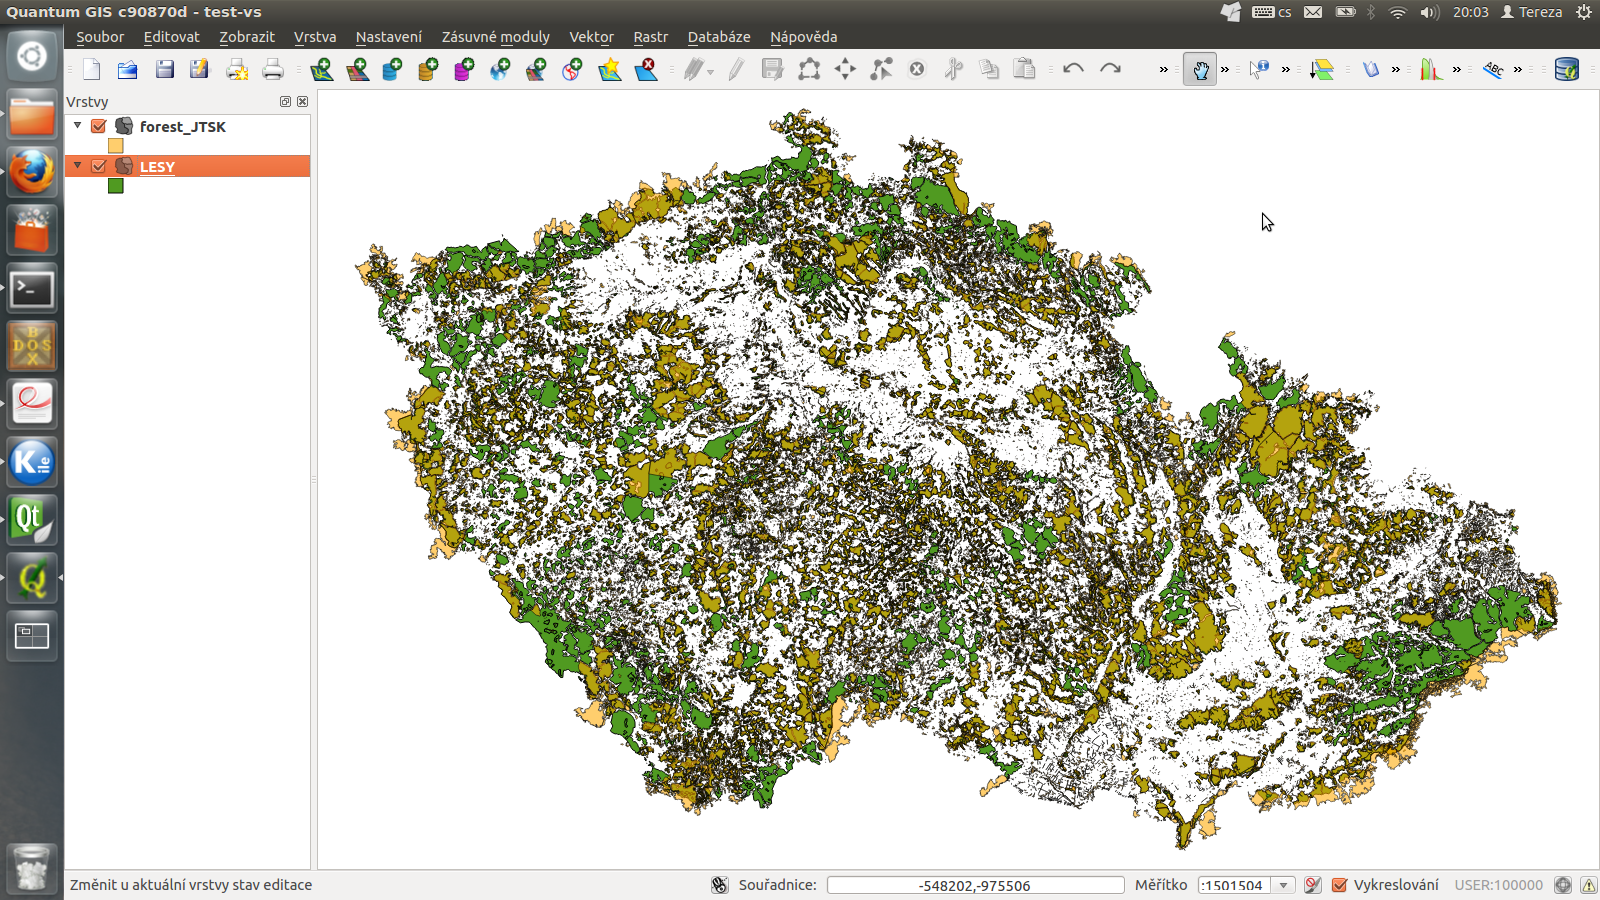
\includegraphics[width=400pt]{./pictures/test-ca1.png}
      \caption{CoverageAlignment - vstupní data}
      \label{fig:ca1}
  \end{figure}

  \begin{figure}[H]
    \centering
      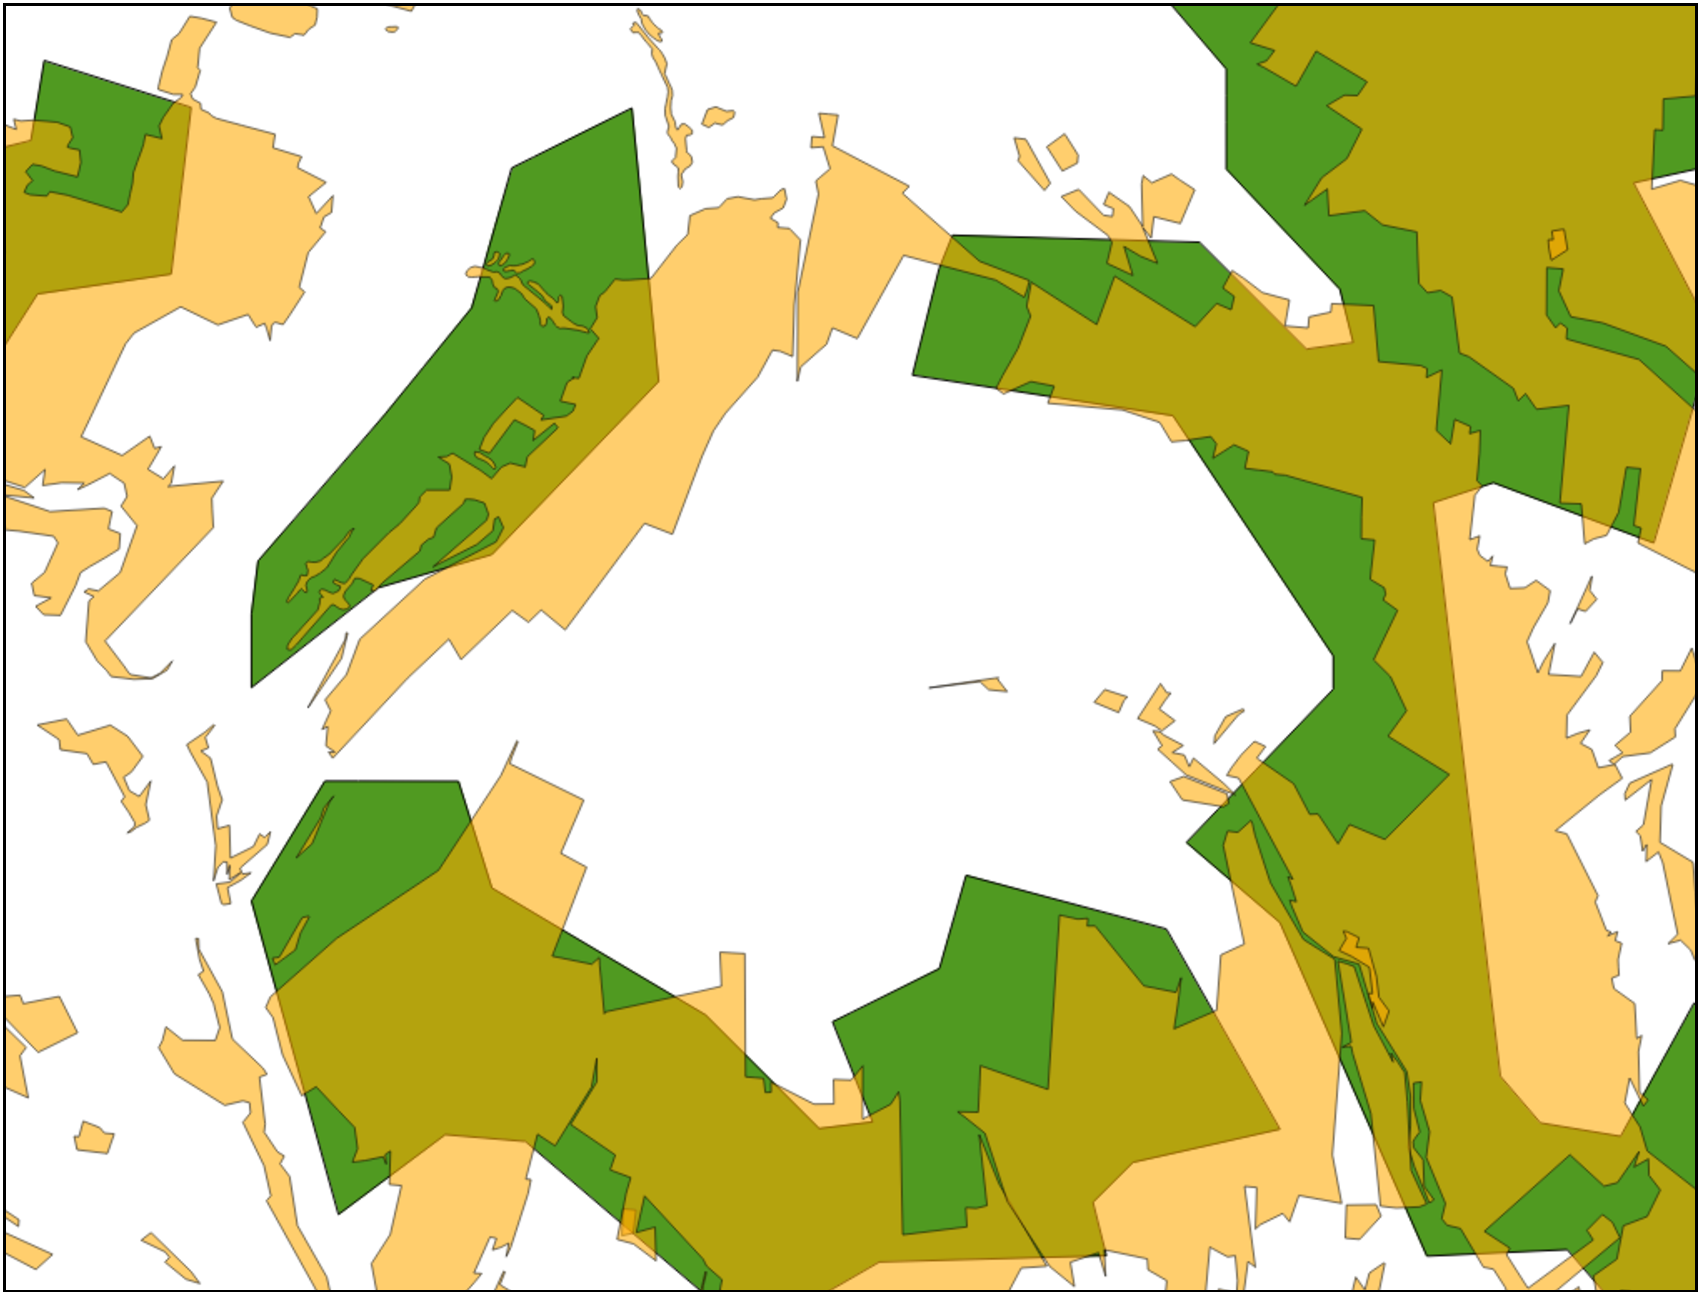
\includegraphics[width=360pt]{./pictures/test-ca2.pdf}
      \caption{CoverageAlignment - před zarovnáním}
      \label{fig:ca2}
  \end{figure}

  \begin{figure}[H]
    \centering
      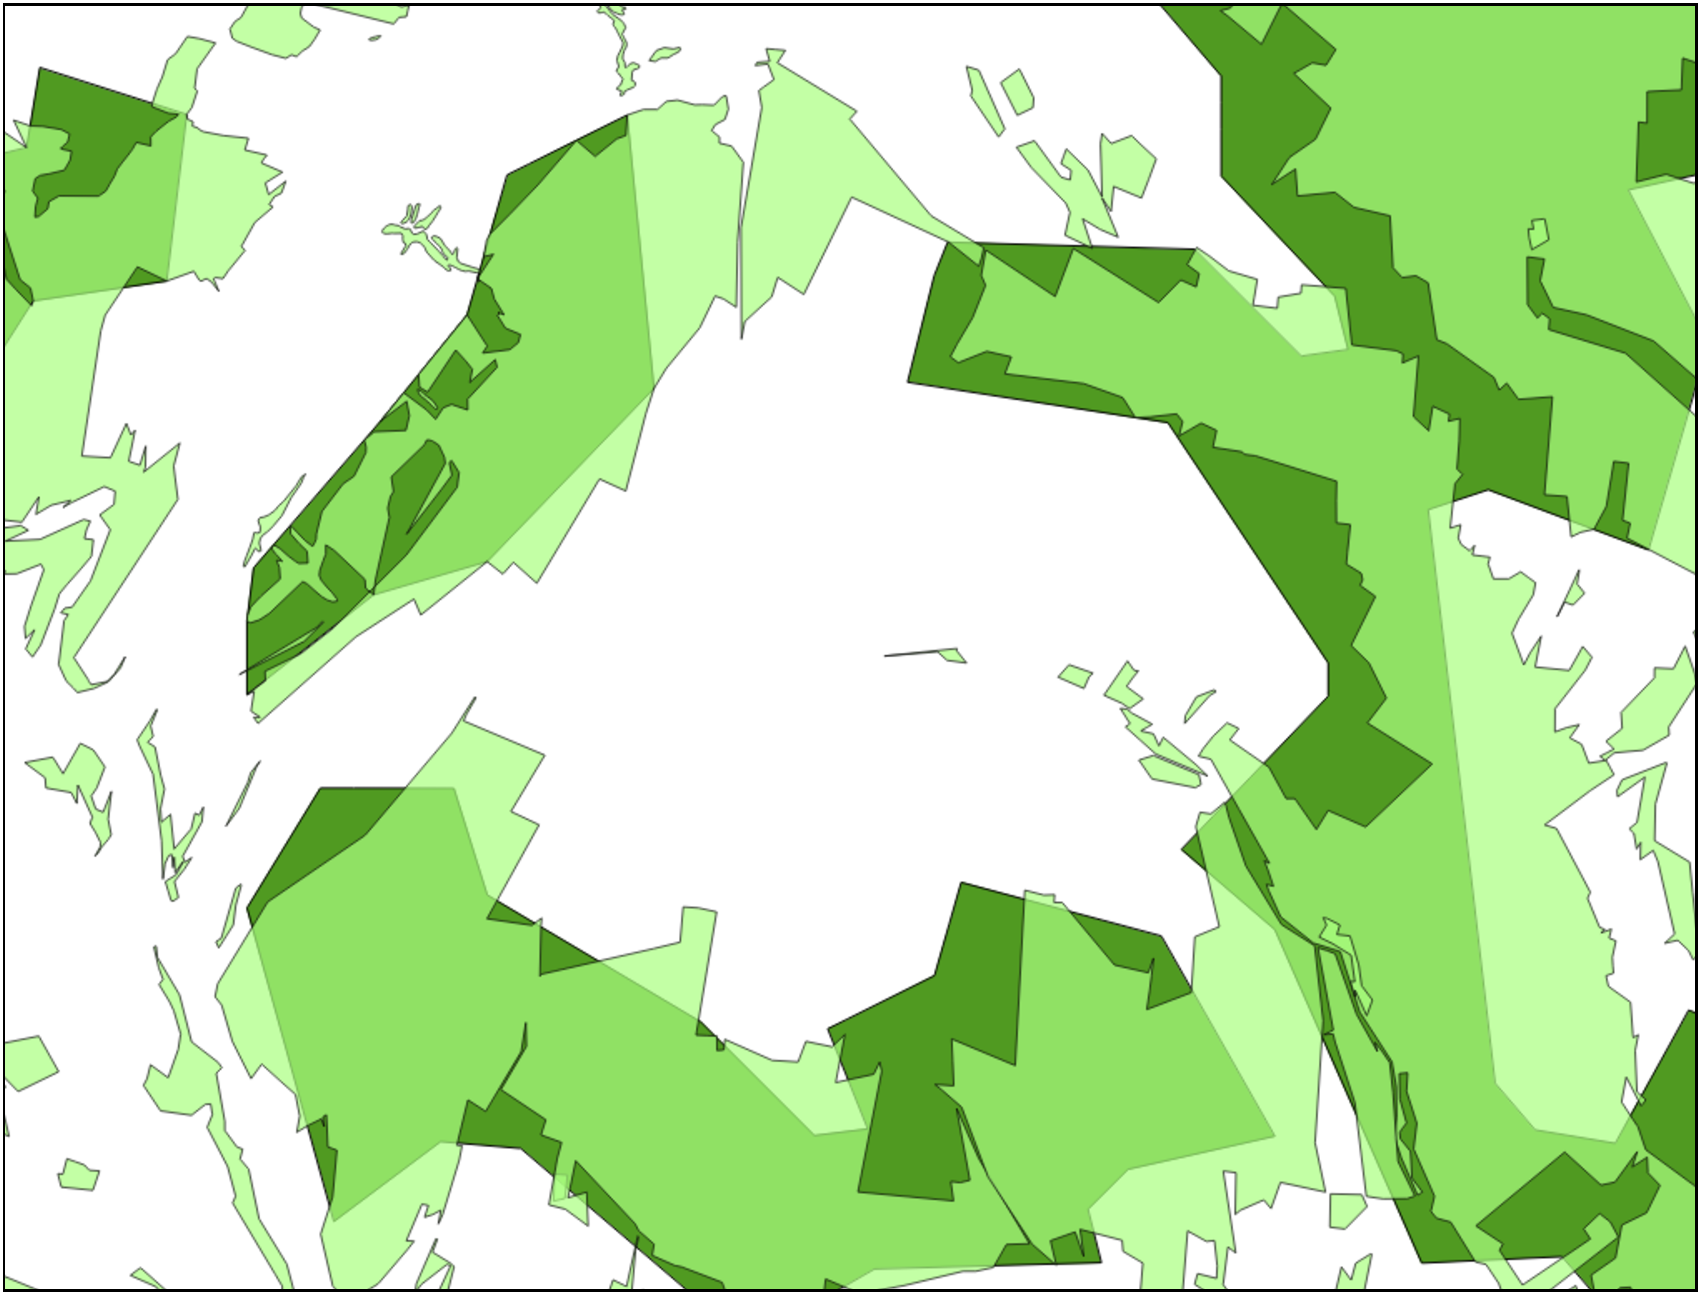
\includegraphics[width=360pt]{./pictures/test-ca3.pdf}
      \caption{CoverageAlignment - po zarovnání}
      \label{fig:ca3}
  \end{figure}

  \begin{figure}[H]
    \centering
      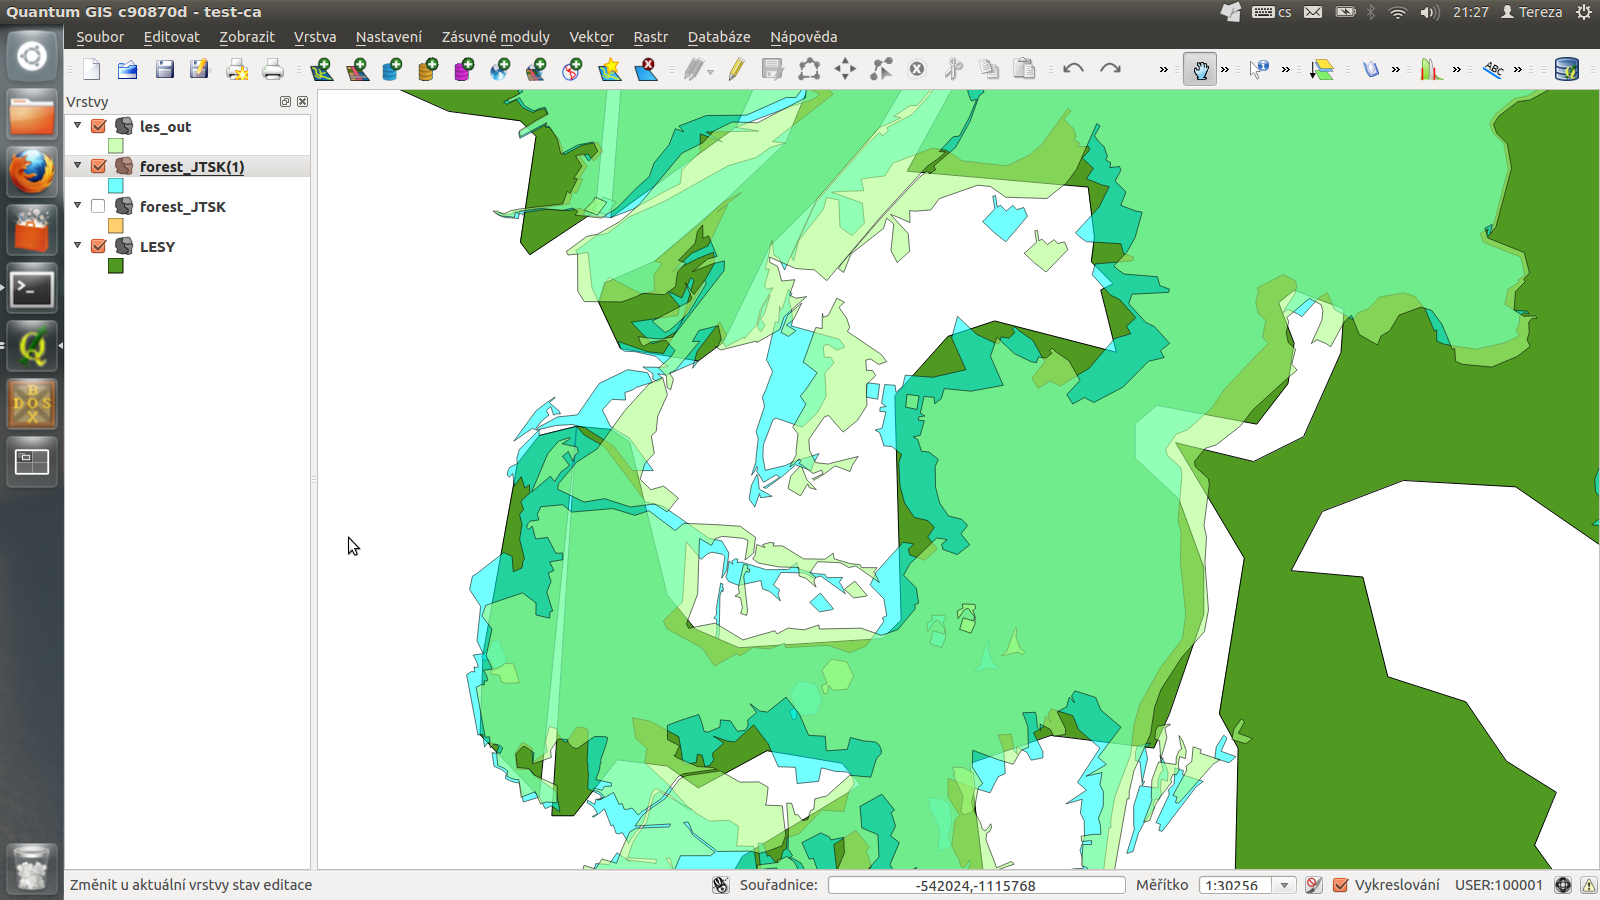
\includegraphics[width=400pt]{./pictures/test-ca4.png}
      \caption[CoverageAlignment- porovnání]{CoverageAlignment 
	- porovnání zarovnání s~toleranční vzdáleností 500 a~1000 m}
      \label{fig:ca4}
  \end{figure}

\section{LineMatcher}
\label{ukazky-lm}

  \begin{figure}[H]
    \centering
      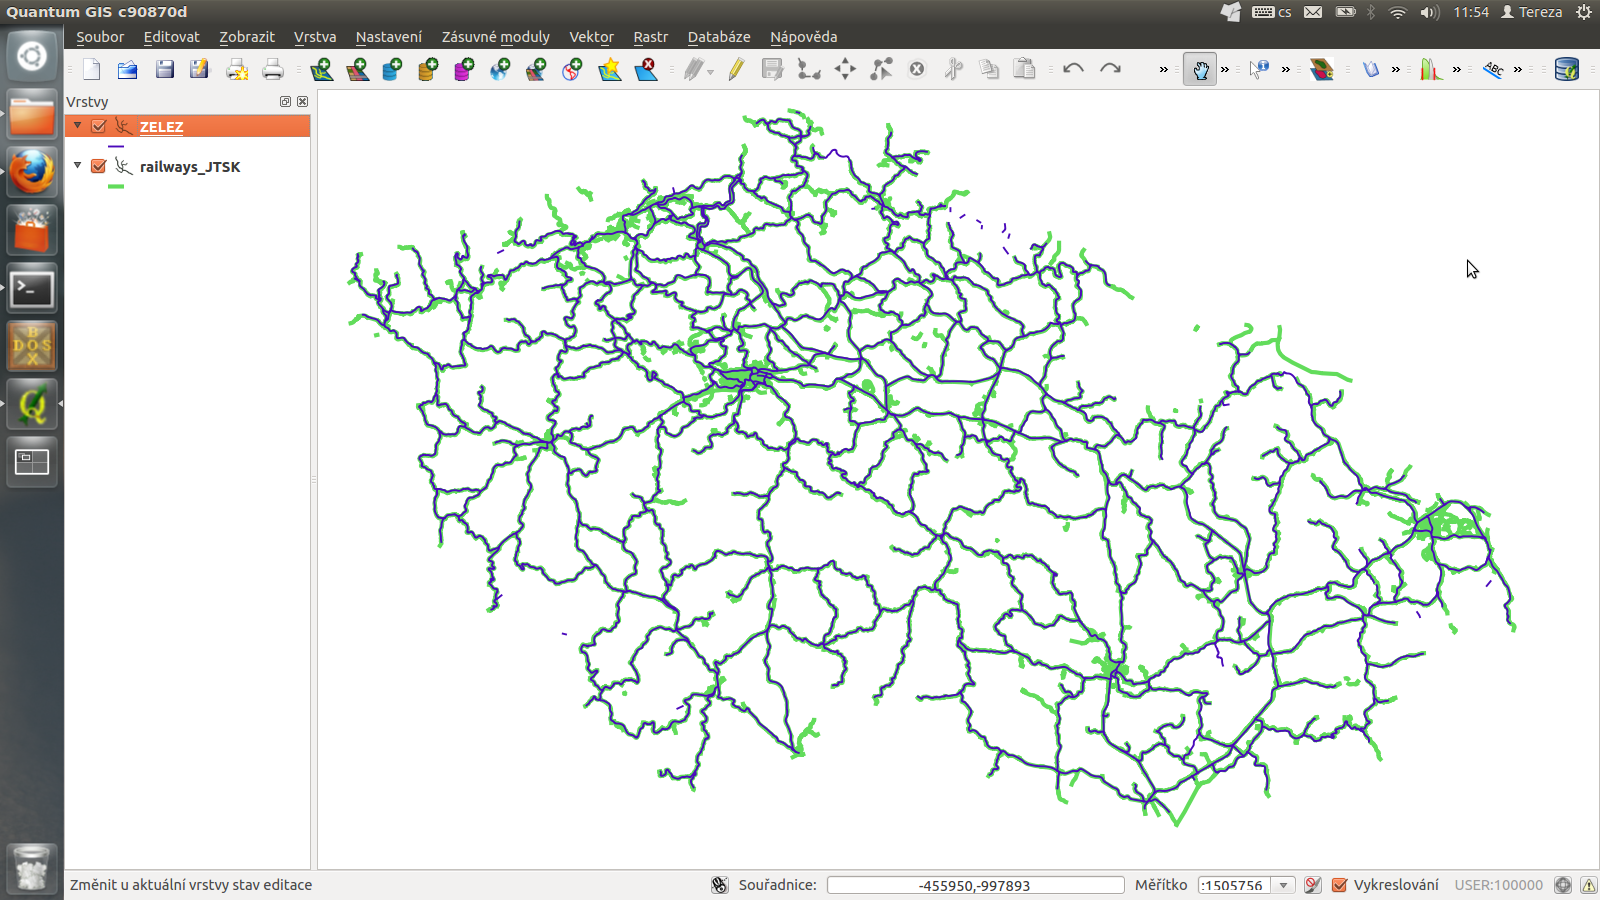
\includegraphics[width=400pt]{./pictures/test-lm1.png}
      \caption{LineMatcher - vstupní data}
      \label{fig:lm1}
  \end{figure}

  \begin{figure}[H]
    \centering
      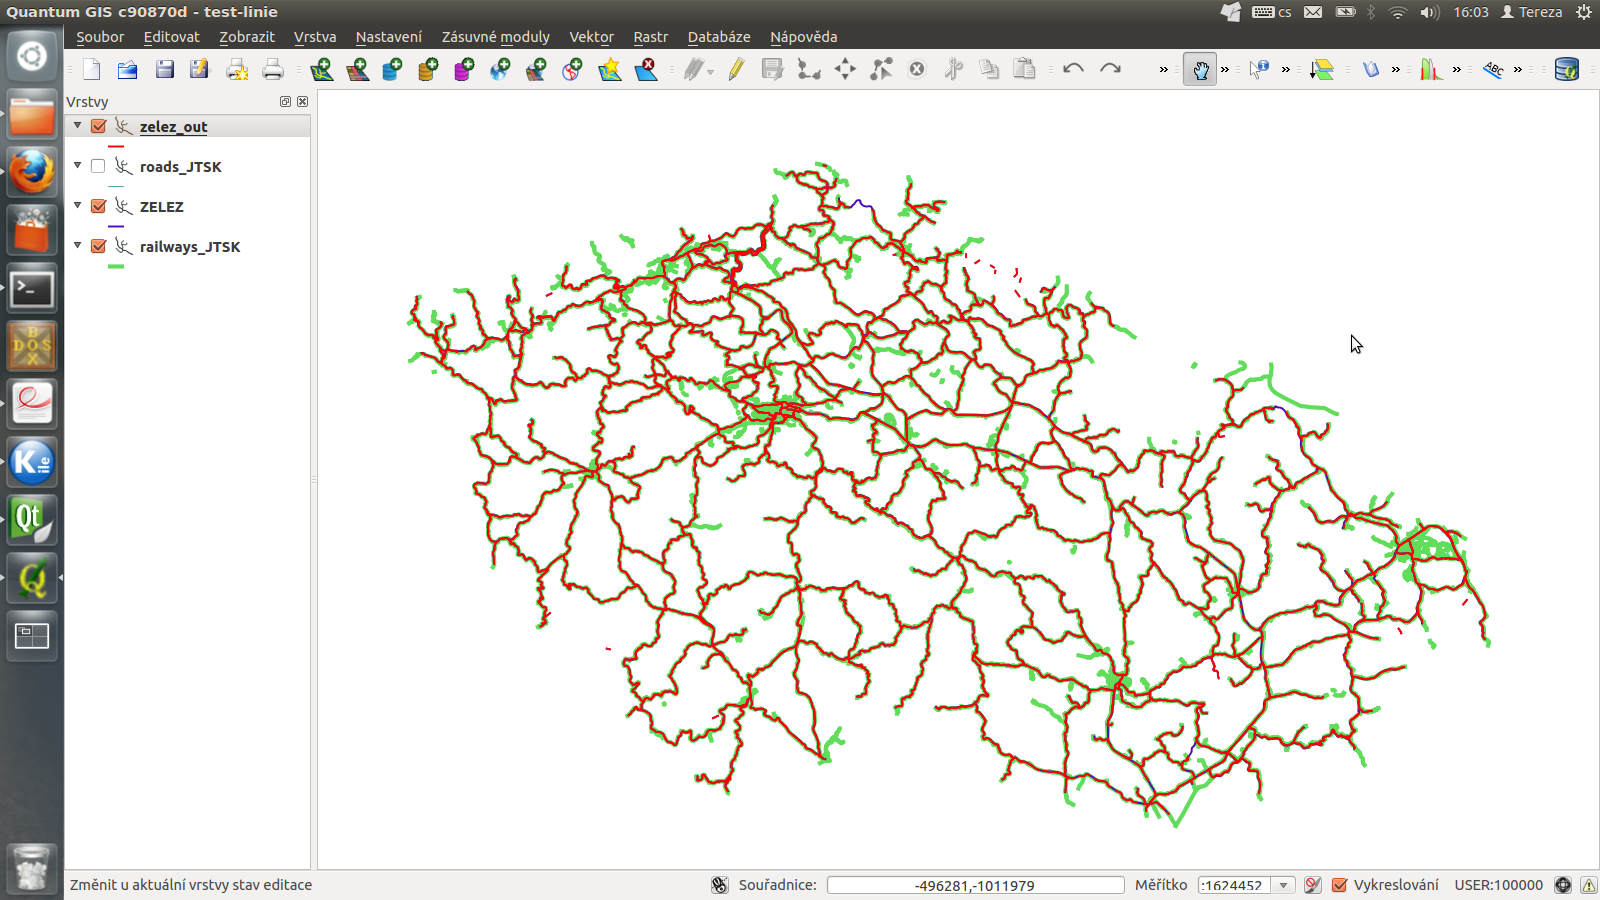
\includegraphics[width=400pt]{./pictures/test-lm2.png}
      \caption{LineMatcher - výsledek}
      \label{fig:lm2}
  \end{figure}  

  \begin{figure}[H]
    \centering
      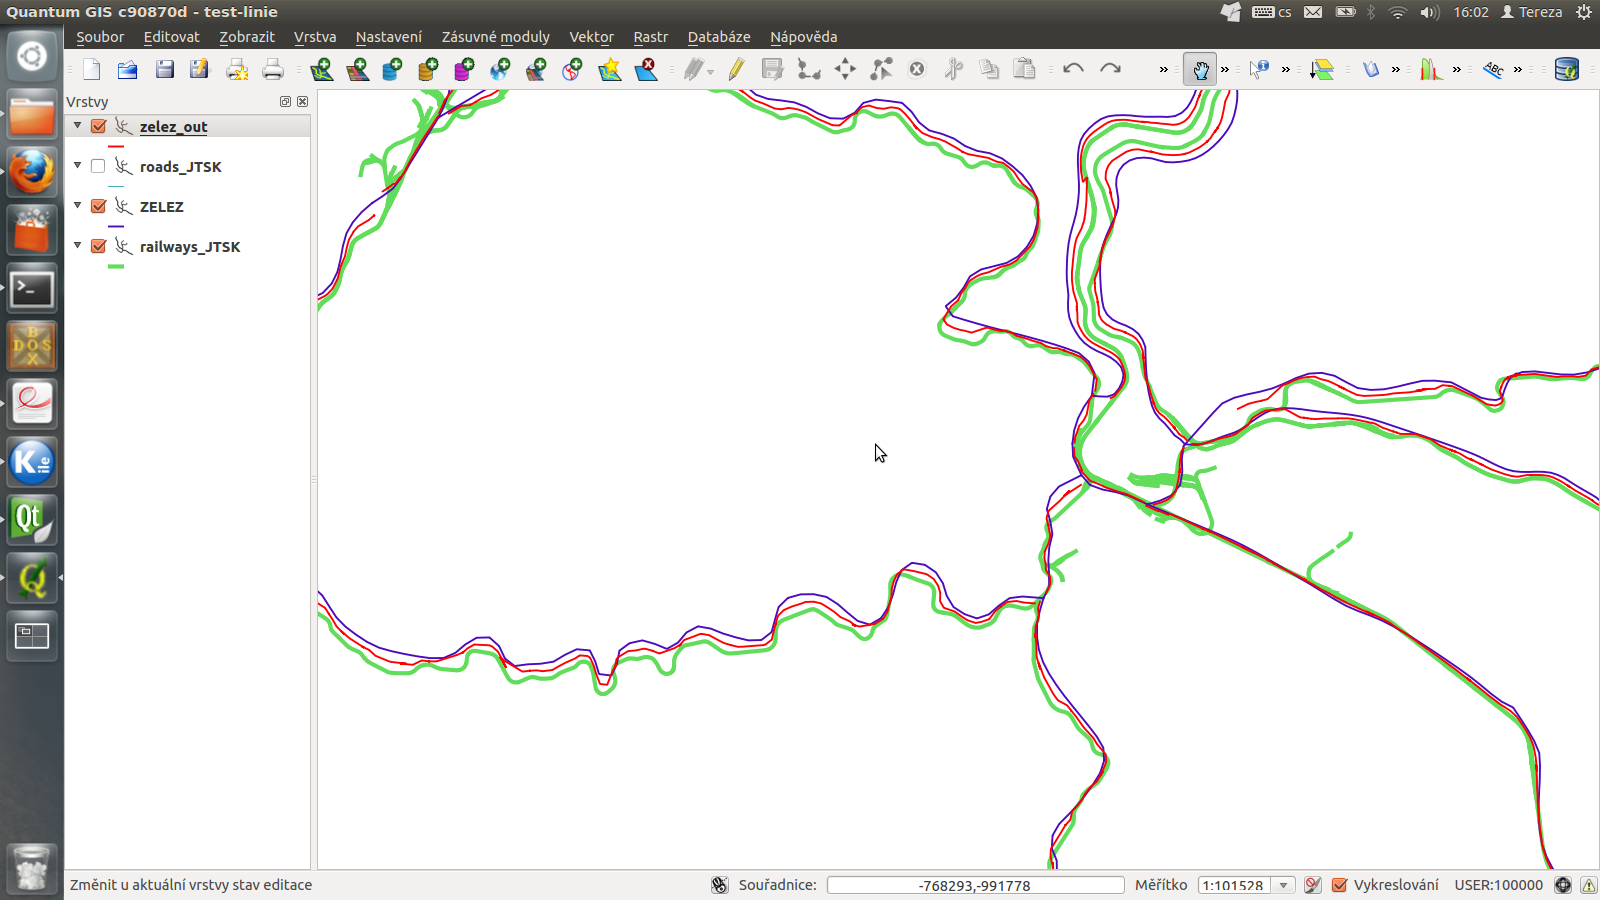
\includegraphics[width=400pt]{./pictures/test-lm3.png}
      \caption{LineMatcher - detail}
      \label{fig:lm3}
  \end{figure}  

%%%%%%%%%%%%%%%%%%%%%%%%%%%%%%%%%%%%%%%%%%%%%%%%%%%%%%%%%%%%%%%%%%%%%%%%%%%%%%%%%%%
%%                 PŘÍLOHA - OBSAH CD                                            %%
%%%%%%%%%%%%%%%%%%%%%%%%%%%%%%%%%%%%%%%%%%%%%%%%%%%%%%%%%%%%%%%%%%%%%%%%%%%%%%%%%%%
\chapter{Obsah CD}
\label{priloha-obsahCD}